\section{研究方法}

%%%%%%%%%%%%%%%%%%%%%%%%%%%%%%
\subsection{理论模型:分布共享数据}

%%%%%%%%%%%%%%%
\begin{frame}{分布共享数据 (I)}
  \todo{图: 分布共享数据服务}
\end{frame}
%%%%%%%%%%%%%%%
\begin{frame}{分布共享数据 (II)}
  分布数据一致性
\end{frame}
%%%%%%%%%%%%%%%
\begin{frame}{分布共享数据 (III)}
  \begin{center}
    \textcolor{blue}{\large 基本定位: 传统概念应用于新型平台}
  \end{center}

  \vspace{0.20cm}
  \begin{center}
    分布共享数据服务: 分布共享内存模型 + 分布数据系统
  \end{center}
\end{frame}
%%%%%%%%%%%%%%%
\begin{frame}{分布共享内存 (I)}
  \begin{figure}
    \begin{subfigure}{0.50\linewidth}
      \centering
      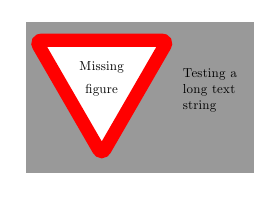
\includegraphics[width=0.50\textwidth]{figures/figure-placeholder.png}
      \caption{共享内存系统.}
    \end{subfigure}%
    \begin{subfigure}{0.50\linewidth}
      \centering
      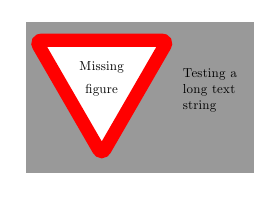
\includegraphics[width=0.50\textwidth]{figures/figure-placeholder.png}
      \caption{分布内存系统.}
    \end{subfigure}
    \caption{多处理器系统体系结构.}
  \end{figure}
\end{frame}
%%%%%%%%%%%%%%%
\begin{frame}{分布共享内存 (II)}
  分布内存系统实例: 按系统耦合度分类
\end{frame}
%%%%%%%%%%%%%%%
\begin{frame}{分布共享内存 (III)}
  \begin{center}
    分布共享内存: 在\textcolor{blue}{分布内存}之上提供\textcolor{blue}{共享内存}的假象
  \end{center}

  \todo{图: 分布共享内存 (from Kai Li)}
\end{frame}
%%%%%%%%%%%%%%%
\begin{frame}{分布共享数据 (IV)}
  问题空间: 传统问题, 新平台, 新挑战
\end{frame}
%%%%%%%%%%%%%%%%%%%%%%%%%%%%%%
\subsection{技术途径: 三维框架}
